\section{Issues of Tizen before 4.0}\label{S_IssueBefore4}

Tizen before 4.0 has a build project for each profile: i.e., Mobile, Wearable, TV, IVI, and Common, which has its own binary repository.
Such binary repositories are not disjoint; there are packages with duplicated names across profiles.
Thus, we cannot compose a software platform with packages of different profiles because the inter-package dependency chain of a profile is not compatible with that of others.
For example, with packages \texttt{A}, \texttt{B}, and \texttt{C}, present in all profiles, where \texttt{A} and \texttt{B} depends on \texttt{C}, we cannot install \texttt{A} from Mobile and \texttt{B} from TV because we cannot install two instances of \texttt{C} from both profiles.
Note that Common profile is simply yet another profile and does not represent common part of others.


Creating a new device type, which happens very frequently with IoT and edge devices, has required to define a new profile and its dedicated build project.
This is not a unique issue of Tizen; Android, dominant for mobile phones, and Yocto~\cite{Streif:2016:ELS:3051933}, popular for IoT devices, also require an independent build project for each device prototype.
For each build project, the infrastructure is required to build the whole packages and developers are required to build and test the packages.
This incurs redundant workloads proportional to the number of device types.
Even if the same source codes are shared across profiles, the whole packages are built repeatedly, which is already too expensive with only five profiles.


Frequently prototyping new device types significantly multiplies such workloads, making it intractable.
Administrators do not allow creating new profiles in the already overloaded infrastructure, where developers and managers keep complaining about the latency.
Besides, creating a new profile has been too difficult for non-build-expert developers.
It requires to fully understand low-level system software packages and the underlying mechanisms of build systems.


\section{Design of Tizen:Unified}\label{S_ach_build_unif}

We have achieved the unification in April, 2017.
We have removed per-profile build projects and provided a single build project and binary repository for all.
The objectives of the unification includes: a) shorter build latency by eliminating duplicated builds; thus, making affordable to support more profiles, b) allowing to create arbitrary profiles from a single shared binary repository, and as a results of a) and b), c) allowing to create new profiles on-the-fly without rebuilding packages, enabling the next big step, configurable Tizen.


There are two major rules to achieve the unification:
\begin{itemize}
\item In build-time, build processes (build scripts, compilers, and build systems including OBS~\cite{19OBS_URL} and GBS~\cite{17GBS2014TizenURL}) should be agnostic to the profile except for the architecture: e.g., \textit{armv7l} and \textit{x86\_64}.
However, processes may identify the profile at install-time, boot-time, or run-time.
\item Every single binary package (i.e., RPM for Tizen) should be able to co-exist in a single repository with other packages as long as the packages have the same architecture.
\end{itemize}

With the completion of the unification, these rules have been applied for all Tizen packages.
The build system is configured to enforce the rules automatically so that any violating changes cannot affect the system since Tizen 4.0~\cite{2Ham2017TDC}.


For the unification, the huge number of software packages itself has been a significant challenge; e.g., Tizen 3.0 Common profile has 822 source packages~\cite{2Ham2017TDC}.
When we have started planning Tizen:Unified in July, 2016, we have discovered 134 source packages disobeying the rules.
When we have started refactoring with a small team of four developers in November, 2016, the number of such packages has increased to 171.
Another challenge is the regression, where a complying package becomes not complying.
We have observed multiple cases of such regressions, both regressions of the refactored packages and natively complying packages.


Ideally, refactoring is better executed by main contributors of the package.
However, it requires the main contributors to fully understand the concept of Tizen:Unified, the mechanisms of build systems under their own workloads and tight schedules.
During the early phase of the project, as a pilot program, we have tried the ideal method with few small groups.
As the result, we have learned the following points:


\begin{itemize}
\item We should not expect developers to fully understand the build system and inter-package dependencies.
They are users of the build system and a good build system should not require users to understand the system itself.
\item It is extremely difficult to ensure that the rules are kept during active development where new commits are applied daily if not hourly.
\item Applying yet another coding rule requires additional burden to developers.
Even if the need is justified to team leaders and main contributors, it is often not enough for them to put additional efforts to prevent others from breaking the rules or to review more carefully.
Moreover, we cannot enforce the rules with the infrastructure until every package follows the rule perfectly because any disobeying package will break the build.
\end{itemize}

As a conclusion, we have decided to do all the refactoring with Tizen:Unified members except for a few packages (Chromium, EFL, and input systems) with much complicated issues that require to rely on their own main contributors.
During the progress of Tizen:Unified project, to detect any attempts of regression, we have developed a gerrit~\cite{6GerritURL} monitoring service that reviews incoming commits and finds any possible regressions.


We categorize packages to refactor into the following types:
\begin{itemize}
\item \textbf{Type-A.} The build script is aware of profiles. It may use different source files or code blocks statically (usually with \texttt{\#ifdef} or \texttt{\#if}) per the profile.
\item \textbf{Type-B.} Multiple git repositories generate packages with a common name. For example, both \texttt{mobile/efl-config.git} and \texttt{wearable/efl-config.git} had generated efl-config.
\item \textbf{Type-C.} At build-time, the package depends on packages that generates different build environments per profile.
\end{itemize}

We have observed a lot of useless dependencies on the profiles or device types and removed them immediately.
We also have had cases where the dependencies are easily removed by using configuration files in \texttt{/etc}. 


\subsection{Runtime profile identification}\label{SS_RUntimeProfileId}

If we cannot avoid per-profile behaviors, applying the runtime profile identification is recommended.
This is recommended because it allows using the same binary across different profiles avoiding installing different binaries per profile.
The only more recommendable method is to behave exactly same regardless of the profile definition itself, which is often impossible.
Many Type-A cases are resolved by this.

\renewcommand{\tablename}{Code}
%% TODO : Check the template if this is allowed.
\begin{table}

\begin{center}
\line(1, 0){250}
\end{center}
\vspace{-0.1cm}

\hspace{0.5cm}\begin{BVerbatim}[baseline=c]
#ifdef PROFILE_MOBILE
    Do_mobile_action();
#else
    Do_common_action();
#endif
          (a)
\end{BVerbatim}
%% \quad$\parallel$\quad
\begin{BVerbatim}[baseline=c]
  ||  if (get_profile() == MOBILE)
  ||      Do_mobile_action();
  ||  else
  ||      Do_common_action();
  ||       
  ||            (b)
\end{BVerbatim}

\vspace{-0.1cm}
\begin{center}
\line(1, 0){250}
\end{center}
\vspace{-0.2cm}

\captionsetup{labelformat=simple,labelsep=period}
\caption{(a) Type-A code with \texttt{\#ifdef} and (b) refactored code}\label{TABLE_CODE_IFDEF}
\end{table}

In order to allow runtime identification, we have used a Tizen API to detect the profile and removed all preprocessor conditionals related. Code~\ref{TABLE_CODE_IFDEF} shows a simple example where such refactoring is applicable.

\subsection{Inter-package dependency management}\label{SS_interpkg_dep_mgt}

Sometimes, we have created different binary packages for each profile or device types along with meta packages or virtual packages (RPM capabilities) to make per-profile differences transparent to other packages.


Let us assume that we have a package \textit{X}, which needs to have different binaries for mobile profile.
Then, we can write the build scripts to create a subpackage, \textit{X-profile\_mobile.rpm}.
The first variation of the mechanism is to create \textit{X.rpm} file for other profiles and to create \textit{X-profile\_mobile.rpm} that may act as \textit{X.rpm} by adding the reverse-dependency, \textit{Provides: X}.
With the first variation, \textit{X.rpm} needs to declare that it \texttt{Provides} virtual subpackages such as \textit{X-profile\_common} in order to be explicit for per-profile configurations.
The second variation is to create a meta package, \textit{X.rpm} without any files, but with meta data stating its dependencies on a virtual subpackage, \textit{X-compat}, and to create subpackages of profiles that do \texttt{Provides: X-compat}, which enforces to install one of such subpackages to install \textit{X.rpm}.
Both variations require subpackages to declare \textit{Conflict} statements to prevent installing plugins of different profiles for one main package.


A critical side effect of these mechanisms is that build systems (both OBS~\cite{19OBS_URL} and GBS~\cite{2Ham2017TDC}) are confused by multiple candidates (the subpackages) for inter-package dependency resolutions.
In other words, if \textit{X.rpm} is required by \textit{Y.rpm} while we build \textit{Y.rpm}, the build systems cannot determine whether it should install \textit{X-profile\_mobile.rpm} or the other; they do not accept such ambiguity.
We have resolved such ambiguity with weak dependencies, \texttt{Recommends}, to declare default selection for build systems, which the corresponding open source community (BSSolve and OBS) have accepted.
We have chosen the weak dependency, \texttt{Recommends}, because we can override it with strong dependency, \texttt{Requires}, for other plugins or profile supports while we may provide hints for build systems.
There is a weaker dependency in RPM standards, \texttt{Suggests}; however, we have not used it for this purpose because only human is supposed to use \texttt{Suggests}; thus, we use \texttt{Suggests} for constructing package list GUI only.
Note that having the default package with \texttt{Recommends} at built time does not affect software platforms with different plugin packages because they are shared objects; only their forms (header files) matter, which holds for Tizen native platform binaries.
However, we had exceptions to this, mentioned in the next section, where the contents of external headers (APIs) differ per profile.



\begin{figure}
\centering
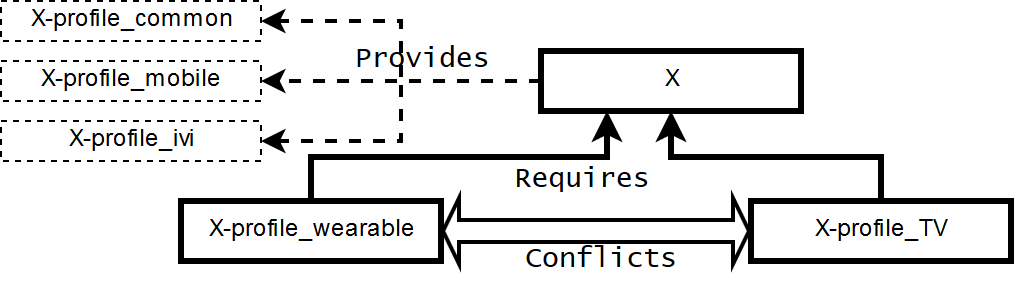
\includegraphics[width=0.98\columnwidth]{figures/Dependency_nonmeta_X.png}
  
\vspace{0.2cm}
  
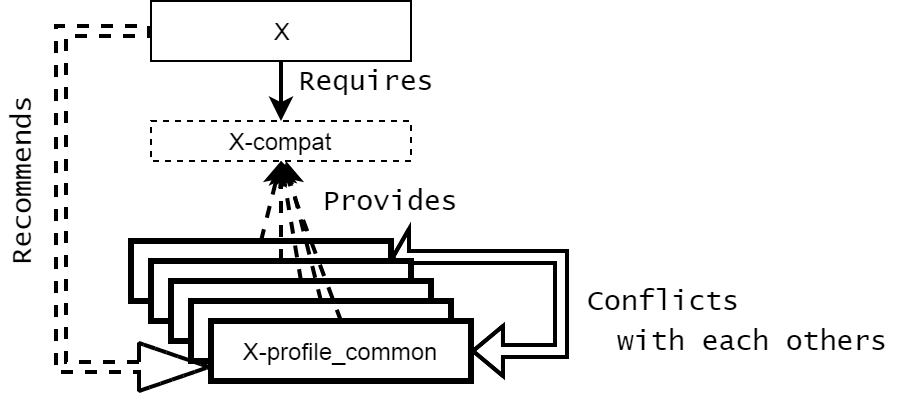
\includegraphics[width=0.98\columnwidth]{figures/Dependency_metaX.png}
% For more control in figure
\caption{The two subpackaging examples supporting different binaries per profile transparently to other packages.}
\label{FIG_TZN_TYPEB_RESOL}
\end{figure}

Fig.~\ref{FIG_TZN_TYPEB_RESOL} elaborates inter-subpackage dependency management mechanism; the top shows the first variation and the bottom shows the second variation.
Note that any packages external to \textit{X} should not explicitly depend on profile plugin subpackages (\textit{*-profile\_*.rpm}).
Such packages should refer to the main package (\textit{X} in Fig.~\ref{FIG_TZN_TYPEB_RESOL}) only and let the package management system handle the rest.


Type-B and Type-C are mostly resolved by declaring inter-package dependencies explicitly after properly refactoring the build scripts and source codes so that per-profile parts are separated into different binary packages.
There are many Type-A cases resolved by this mechanism as well when it is too difficult to apply the mechanism of the Section \ref{SS_RUntimeProfileId}.
It is usually when a profile has completely different source code files, which incurs too large modifications to apply runtime profile identifications.
In such cases of Type-A, we generated different executables for each profile and packaged them into different binary packages, which is often referred as sub packages.
However, for the package management mechanism, there are no differences between packages and sub packages.


\subsection{Inappropriate definitions of APIs}\label{SS_uglyAPI}

Unfortunately, a few developers have written external header files with different function declarations per profile or even provided different header files for different profiles.
There has been even a case where Tizen public API header has different C enum definitions per profile.
In this case, the C enum definitions of mobile have been \texttt{PLAYER\_DISPLAY\_TYPE\_EVAS = 1} and \texttt{PLAYER\_DISPLAY\_TYPE\_NONE = 2} while those of wearable have been \texttt{PLAYER\_DISPLAY\_TYPE\_EVAS = 2} and \texttt{PLAYER\_DISPLAY\_TYPE\_NONE = 1}.
This extreme case has required Tizen public API changes that may make previous applications incompatible with new Tizen versions.
Thus, we have redefined C enum values with unused and unified values and marked old values (1 and 2) as deprecated along with compatibility resolving code that behaves differently for each profile detected in run-time.


For the first case, where profiles have had different function declarations using compiler preprocessor conditionals, we have manually refactored header files removing all preprocessor conditionals.
We cannot apply the mechanism of Section \ref{SS_interpkg_dep_mgt} for headers exposed externally because the depending package (\texttt{X.rpm} in the examples of Section \ref{SS_interpkg_dep_mgt}) cannot be identical for different profiles; profile dependency is no more transparent to external packages!
For the other cases, where different files have been used per profile, we have manually inspected each declaration and merged them into a superset containing all declarations from all profiles.
Then, we have added dummy function definitions for profiles that do not or cannot execute it, determined either at run-time with profile probing APIs or at install-time with different binaries per profile.


\subsection{Workarounds}

There are a few cases where we cannot completely remove the dependencies on profiles or device types from the binary packages except for the plugin subpackages, which do not incur external dependencies.

\begin{itemize}
\item Case 1: Device drivers or kernel binaries require dependencies on device types and often, such dependencies are hardcoded.
\item Case 2: We are not allowed to generalize product or business division specific routines. A business division has required keeping their product specific conditional codes embedded in Tizen while such codes cannot be generally used for other profiles or devices. Although, in principle, this is undesirable as it fragments the source code and damages the readability, this has been something we could not alter.
\end{itemize}

Case 1 includes Linux kernel, which is built and installed for all devices, but their source code repositories or build configuration might differ.
We have applied an altered method of Section \ref{SS_interpkg_dep_mgt} as shown in Fig.~\ref{FIG_TZN_KERNELDEP}.


\begin{figure}
\centering
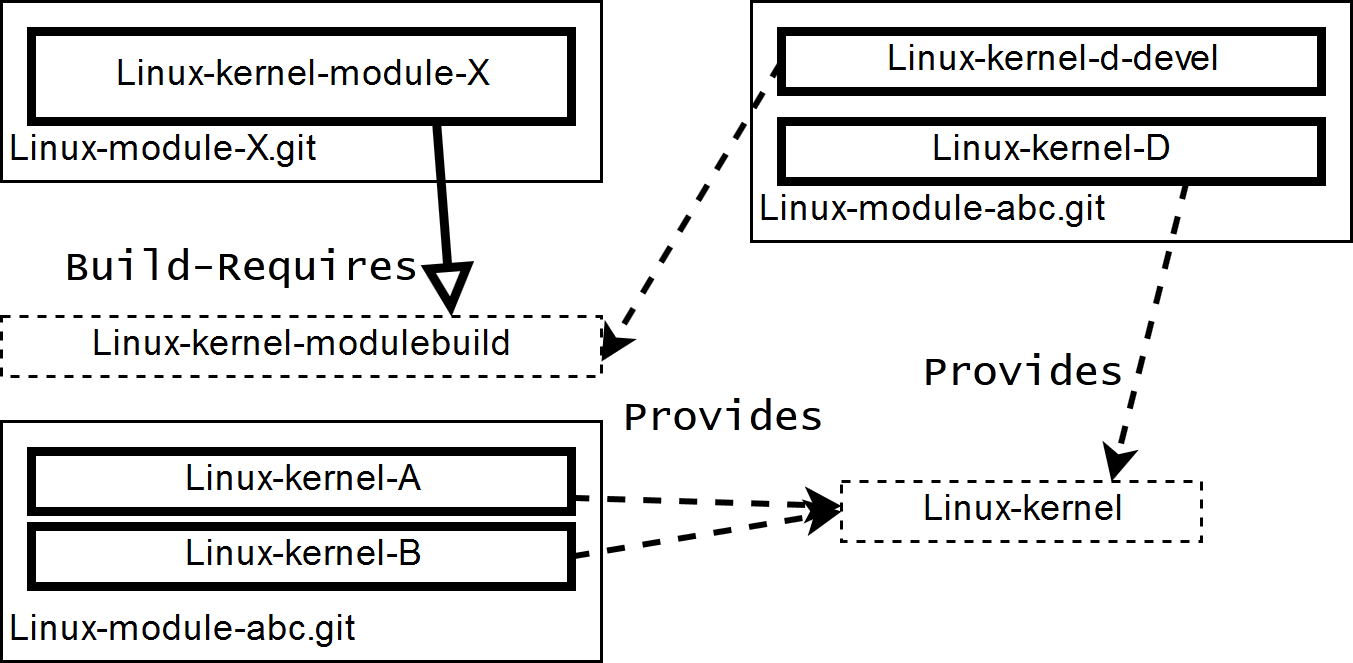
\includegraphics[width=0.95\columnwidth]{figures/KernelDeps_v2.png}
\caption{The altered method of Fig.~\ref{FIG_TZN_TYPEB_RESOL} for Linux kernel}
\label{FIG_TZN_KERNELDEP}
\end{figure}

As shown in Fig.~\ref{FIG_TZN_KERNELDEP}, different Linux kernel binaries from various git source repositories provide the capability of Linux-kernel so that any package or software platform manifests requiring Linux-kernel can be satisfied with one of Linux-kernel binary packages.
However, as mentioned before, we cannot have multiple candidates for a single dependency (or capability in RPM documents) in build time.
Thus, for external kernel module repositories, a representative kernel repository has been chosen to provide the Linux-kernel-modulebuild capability, which is the emulator kernel repository.
Note that we can have a single representative for each Linux kernel version.
Therefore, if there are multiple Linux kernel versions required for a specific Tizen version, we can choose multiple representatives, one for each kernel version.
We may choose multiple representatives without introducing the ambiguity for build systems by specifying kernel versions in kernel modulebuild dependencies.
That is \texttt{BuildRequires: linux-kernel-modulebuild = 4.4.0} and \texttt{Provides: linux-kernel-modulebuild = 4.4.0}  instead of \texttt{BuildRequires: linux-kernel-moduilebuild} and \texttt{Provides: linux-kernel-modulebuild}.


For case 2, we have configured the Tizen main public build systems to ignore any macros related with products or business divisions.
Although we have allowed preprocessor macro conditionals for products and business divisions, as long as the main build system ignores such macros, we can guarantee that the resulting binaries are complying Tizen:Unified.
Simultaneously, with the same source code repositories, a business division may keep their own special source code activated in their own build projects in their own private build systems.
However, codes creating different binaries under the same package names should be discouraged.
Such codes are usually the results of laziness (or overloaded workloads) of developers; they should have used configuration files (.ini files in /etc directory) or accessed Tizen device APIs, probing device type, name, and profiles.
We hope, in some day, such lame codes are totally eliminated.


\subsection{How we have progressed}

Regressions by incoming commits breaking the rules mentioned in the first paragraphs of Section \ref{S_ach_build_unif} have been headaches for the Tizen:Unified project.
Before April, 2017, during the active development of Tizen:Unified project, the build system could not be configured to ignore per-profile build configurations.
Thus, we have constantly monitored incoming Tizen commits with a monitoring service implemented to find any regressions in the rule enforcement.
For the reported regressions, we have intervened the related activities, where we could have successfully dropped or corrected violating commits before being merged.


Once every single package in Tizen has obeyed the given rules of Tizen:Unified, we have removed all per-profile build projects from the infrastructure and unified all Tizen packages into a single build project named \texttt{Tizen:Unified}, which does not allow any dependencies on profile or device types in built-time.
Note that build projects for older versions (e.g., Tizen 2.x or 3.0) are untouched and kept with per-profile basis; however, they are no more actively developed and do not require heavy build workloads as work-in-progress versions.
Another build project, \texttt{Tizen:Base} exists independently in order to reduce the performance impact from cyclic build dependencies of toolchains.
Cyclic build dependencies incur heavy redundant build workloads and are prohibited in Tizen:Unified because it is expected to be rebuilt frequently; most developers contribute to Tizen:Unified daily.
Note that as long as multiple build projects are disjoint (not sharing source repositories) and inter-project dependency is acyclic, there is no build performance problem and on-the-fly configurability.
The traditional per-profile build projects are not disjoint, sharing hundreds of source repositories with each other.


Once Tizen:Unified is completed, we have observed another unexpected advantage that we could have exploited for other projects.
We can add a disjoint build project that does not have cyclic inter-project dependencies without any deterioration on the performance or the configurability.
With this characteristics, we could have created aggressive prototypes quickly without affecting conventional Tizen projects.
An autonomous driving project and an on-device AI platform project require a lot of additional source repositories, well over 100.
Besides, although these projects are based on Tizen, they are not officially Tizen projects and the related packages could have not be included in official Tizen repositories.
By adding a disjoint build project, depending on Tizen:Unified, but outside of Tizen official build infrastructure, Tizen:TAOS (representing Tizen AI OS Support, Tizen Autonomous-driving OS, and Tensor-Aware OS simultaneously), we could have been aggressively prototyping new software platforms.
When there is a new need for yet another variation, a single developer can generate and deploy a new software platform and its binary images to corresponding developers and devices within few hours, which is frequently occurring.
The inter-project dependencies are shown in Fig.~\ref{FIG_TZN_INTERPDEP}.
In Fig.~\ref{FIG_TZN_INTERPDEP}, shaded blocks represent Building Blocks and white blocks represent individual software packages.
Blocks with thick outlines represent mandatory items--subblocks or individual packages of a block--, which means the items are chosen unconditionally if their parent is chosen.
For example, if a parent, \texttt{Graphics}, is chosen, its mandatory item (child), \texttt{2D}, is always chosen.
On the other hand, optional item, \texttt{3D}, is may be omitted even if \texttt{Graphics} is chosen.
Note that unless explicitly declared, a child may be chosen without choosing its parent.
For example, \texttt{3D} or \texttt{2D} may be chosen without choosing \texttt{Graphics}.
If the whole platform has not been unified as in pre-4.0 Tizen, this would have been challenging task because we cannot pick a few packages from a profile and some other packages from another profile simultaneously for a single new project.
Note that this is different from the configurability because the configurability is to configure a system within the official Tizen project.

\begin{figure}
\centering
  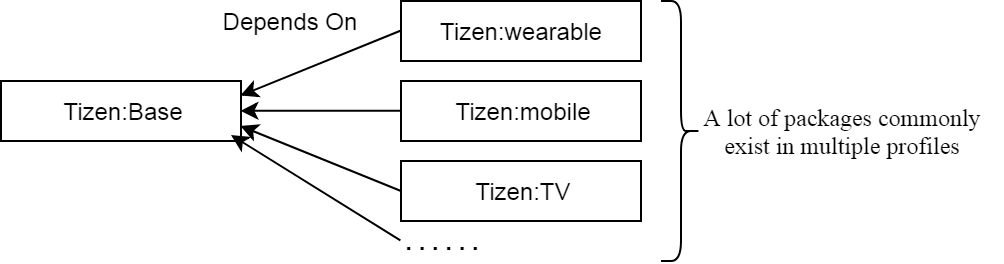
\includegraphics[width=0.95\columnwidth]{figures/InterprojectDeps_Old.png}
  
  \vspace{0.1cm}
  
  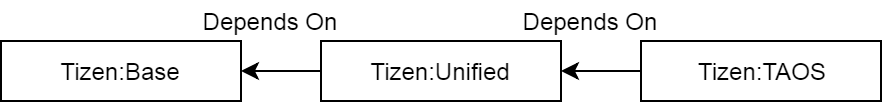
\includegraphics[width=0.85\columnwidth]{figures/InterprojectDeps_New.png}
\caption{Inter-project dependencies of Tizen build projects. The top shows pre-4.0 and the bottom shows 4.0 or later.}
\label{FIG_TZN_INTERPDEP}
\end{figure}

\section{Design of Tizen:Configurability}\label{S_Design_Tizen_Conf}

With the completion of Tizen:Unified project, Tizen has achieved the basic ability to configure a software platform on-the-fly.
Because every single binary package can be located in a single package repository and there is no more ambiguities between package names any more, we can now use package management systems without glitches anymore: zypper, DNF, or yum, which are equivalent to apt in Ubuntu/Debian systems.


For most workstations, PCs, or servers, this degree of configurability may be enough.
However, it is not enough for embedded systems and IoT/edge systems consisting of both devices and software platforms.
For such systems, we need to continuously release and deploy OS images that can be flashed to devices easily without manual labor.
Traditionally, in Tizen, we have been using a tool, MIC, previously named MeeGo Image Creator.
Issues with traditional tools include:

\begin{itemize}
\item Issue 1: It is too difficult to create a new software platform configuration (.ks file) for most users; you need build system experts who understand Tizen and its infrastructure deeply. Thus, it can be practically impossible for most third party developers to create Tizen prototypes.
\item Issue 2: You need your own dedicated Linux workstation to create Tizen images. It would be more appropriate if IoT application developers with an access to web browsers and Tizen Studio~\cite{23tizenstudio2018} can write their own IoT applications and generate proper Tizen OS images for their own IoT devices and applications on the fly.
\end{itemize}

In order to address Issue 1, we have introduced the concept of building blocks and implemented the first draft in \url{https://git.tizen.org/cgit/tools/building-blocks/} in May, 2017.
The concept of building blocks is now the core of Tizen profiles and device type definitions.
It is also the main tool for project managers.
With building blocks, users can create prototypes without the knowledge of thousands of individual Tizen packages or to choose hundreds from them, but with the fewer (about one or two dozens) abstract and easy-to-understand building block names: e.g., Bluetooth, Haptic, and Default-App-Setting.


In order to address Issue 2, we have introduced Tizen Image Creator (TIC), which has the web frontend with node.js.
Analyzing individual packages and generating deployable OS images for the configured prototype is executed in a web server.
Tizen team has opened web service that uses TIC and building blocks as its backend at \url{https://craftroom.tizen.org}: Craftroom.
Craftroom service offers simplified and easier interfaces focused on IoT developers.


\subsection{Building blocks}\label{SS_buildingblocks}

A building block is a meta packages that designates mandatory packages and optional packages.
As a meta package, it does not have its own files, but has dependency relation information consisting the list of mandatory or optional packages.
A mandatory package is an individual Tizen package or another build block that is installed if the corresponding building block is chosen.
An optional package is an individual Tizen package or another building block to be shown in the user interface if the corresponding building block is chosen.
Unlike mandatory packages, optional packages are not automatically chosen with the corresponding building block.


\begin{figure}
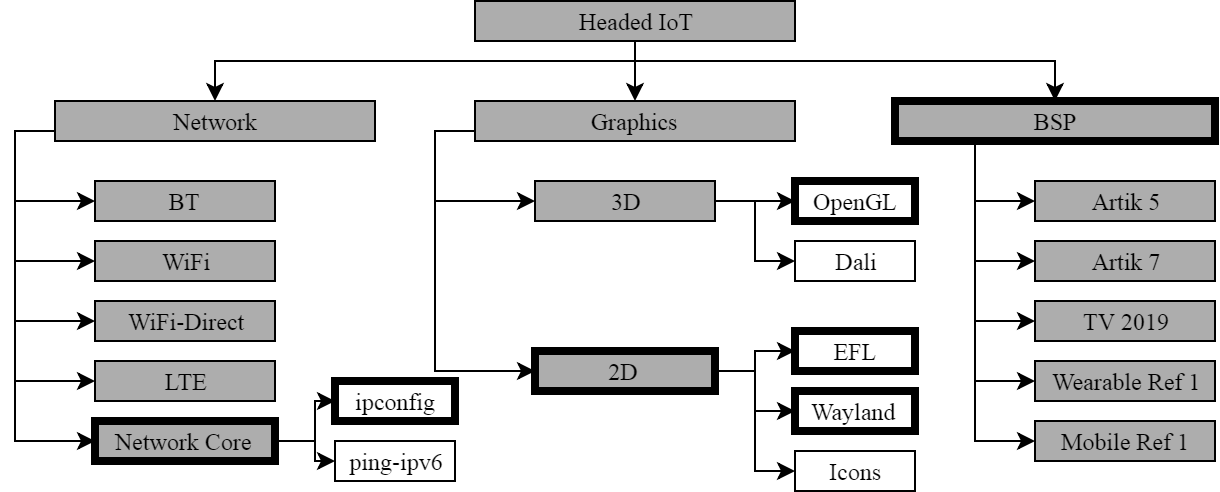
\includegraphics[width=0.95\columnwidth]{figures/BBExample.png}
\caption{Example of building block hierarchy}
\label{FIG_TZN_BBHier}
\end{figure}

Building blocks have the hierarchy between the blocks that can be expressed as a tree with a root node and a leaf node is an individual Tizen package of a empty building block.
Fig.~\ref{FIG_TZN_BBHier} shows an illustrative example of building blocks as a tree.
However, please note that the actual definitions of build blocks are far more complex with a lot of building blocks and individual packages.


In Fig.~\ref{FIG_TZN_BBHier}, boxes filled with gray represent building blocks.
Boxes without gray filling represent individual Tizen packages.
Although most of building blocks are supposed to contain individual Tizen packages, we omitted to simplify the figure.
Boxes with solid thick outlines represent mandatory packages.
Boxes with dashed outlines represent optional packages.
The root node, \texttt{Headed IoT} does not belong to any other building blocks; thus, it is neither mandatory nor optional.


\begin{figure*}
\centering
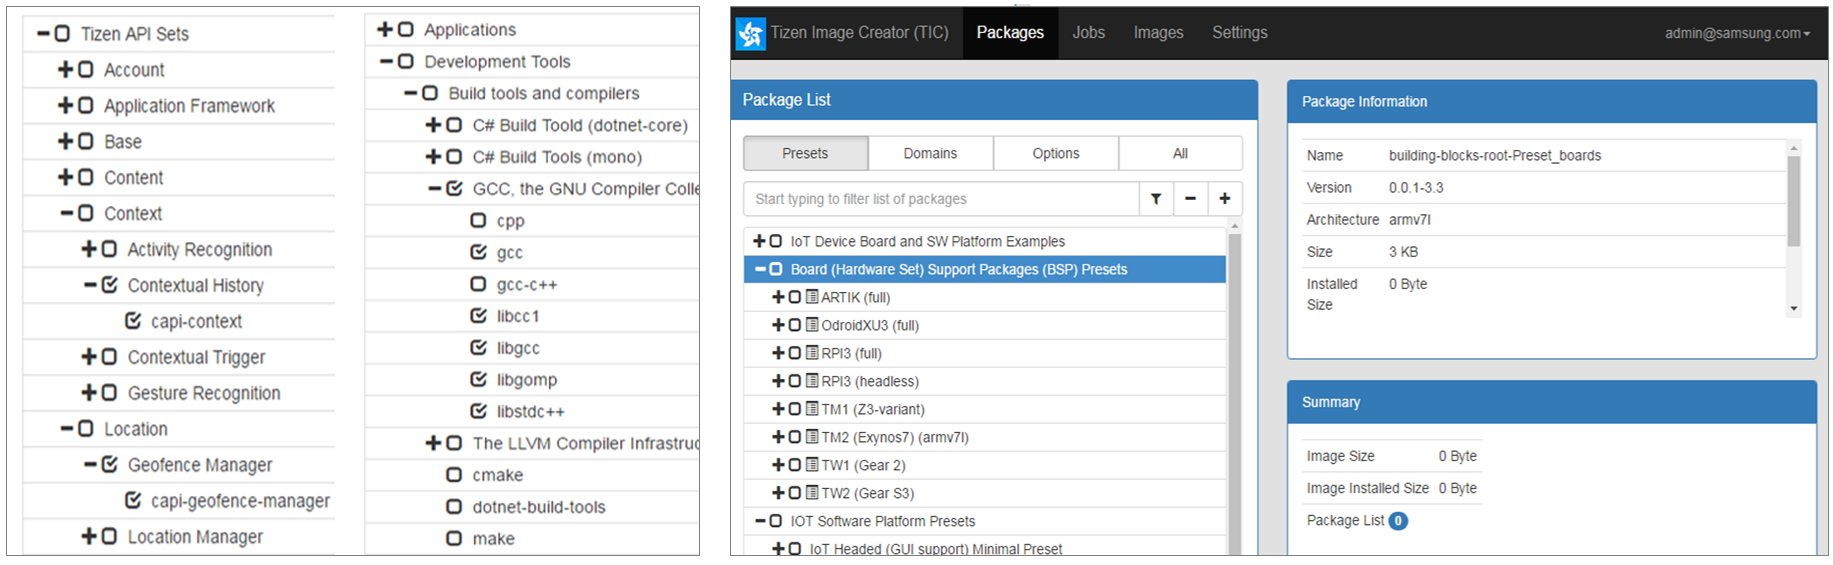
\includegraphics[width=0.96\textwidth]{figures/tic_pkglist_domains_options_presets.png}
\vspace{-0.1cm}
\caption{Building Block hierarchy of May 2017 draft (left) and TIC screenshot where users may choose presets (right)}
\label{FIG_TZN_TIC_SCRSHOT}
\vspace{-0.1cm}
\end{figure*}

%\begin{figure}
%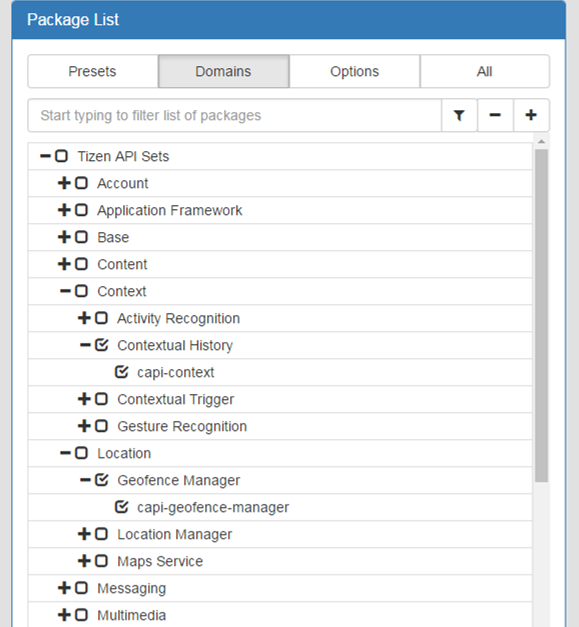
\includegraphics[width=0.47\columnwidth]{figures/tic_pkglist_domains.png}
%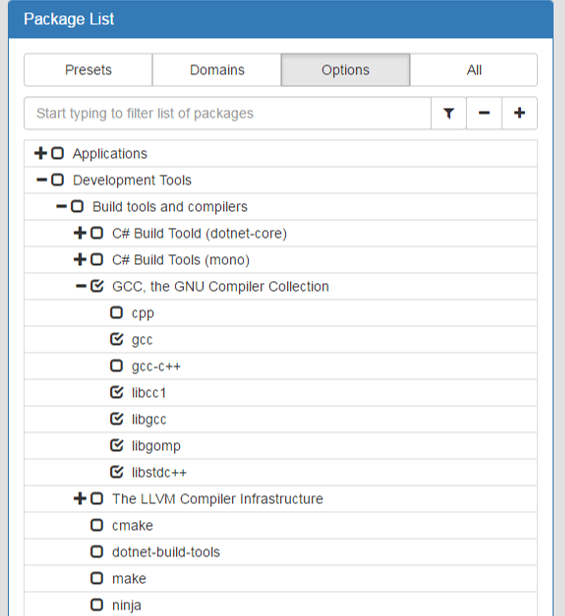
\includegraphics[width=0.47\columnwidth]{figures/tic_pkglist_options_cut.png}
%\caption{Building block hierarchy of May 2017 draft}
%\label{FIG_TZN_TIC_SCRSHOT1}
%\end{figure}

Note that non-hierarchical dependency relations between building blocks are not shown in the figure; e.g., \texttt{TV 2019 Requires 3D}. The hierarchy of building blocks is defined in order to visualize building blocks for users.
The left side of Fig.~\ref{FIG_TZN_TIC_SCRSHOT}, shows how the hierarchy generates building blocks lists for users with TIC, which is to be elaborated in the next section.


In order to make the definitions of building blocks highly readable to project managers and developers and to make the resulting relations consistent, there are a list rules in writing building blocks along with a rule checker that breaks generating building block packages if there is a rule break.
The rule is enforced by a rule checker that is implemented to generate build breaks if there is any violations.
Because the list of rules is too lengthy to be described in this paper, please refer to \cite{7TizenBBRuleURL} for the full list.


%\begin{figure*}
%\centering
%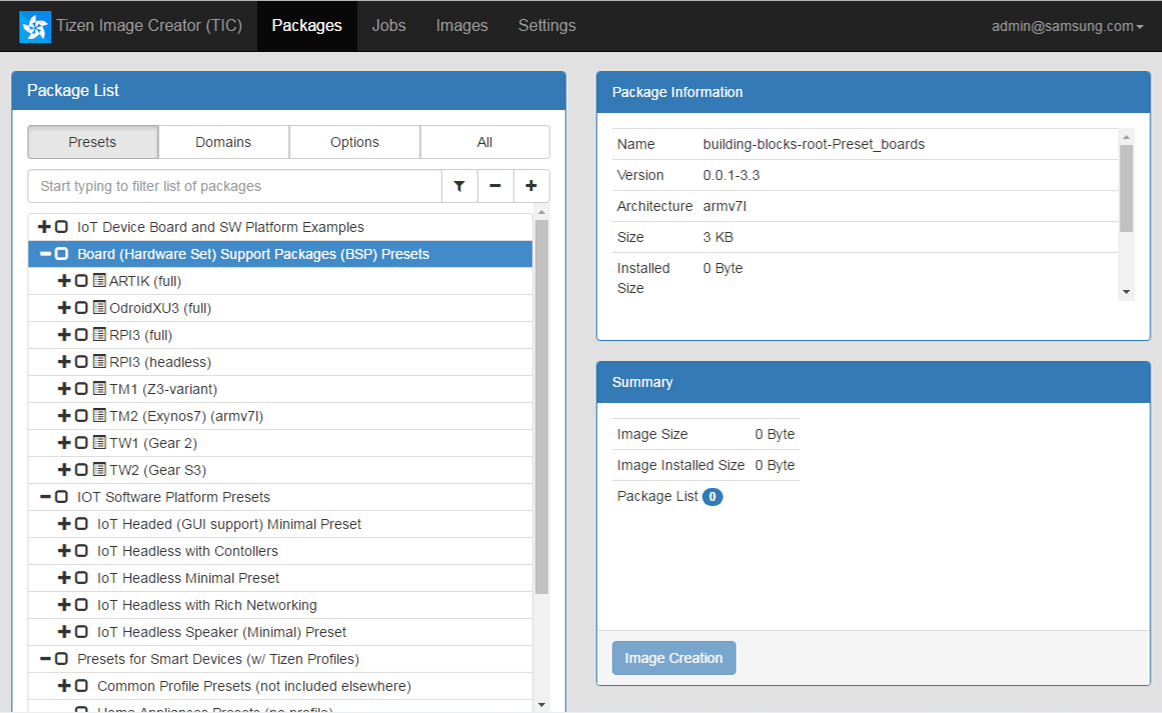
\includegraphics[width=0.80\textwidth]{figures/tic_presets.png}
%\caption{TIC screenshot where users may choose presets}
%\label{FIG_TZN_TIC_SCRSHOT2}
%\end{figure*}

\subsection{Tizen Image Creator (TIC)}\label{SS_TIC}

Tizen experts can prototype software platforms easily with building blocks.
However, third party developers or novice developers require more user-friendly methods than writing a KickStarter~\cite{9TizenKSGitURL} \texttt{.ks} file.
With web application experts, we have developed TIC, which visualizes building blocks and individual packages with their relations and capabilities and configures platforms.


The right-hand side of Fig.~\ref{FIG_TZN_TIC_SCRSHOT} is a screenshot of TIC in a web browser.
There are three categories of building blocks: \texttt{Presets}, \texttt{Domains}, and \texttt{Options}.
\texttt{Presets} provide predefined sets of building blocks and individual packages before actually choosing blocks in Domains or Options.
For example, users may start prototyping a TV platform with a TV Preset, which has all basic features of TV.
In TIC interface, users can review the currently selected blocks and  the currently configured software platform as well.


\texttt{Domains} are building blocks defined by Tizen API sets.
\texttt{Options} are additional blocks that may help development, but are not supposed to be deployed to actual products: e.g., debugging tools, text editors, and profiling tools.


When users have completed configuring the software platform, they may order TIC to create the corresponding OS image file in the server so that they can download the file for deployment a few minutes later.
Users may define additional binary package repositories so that they may add their own custom binaries.
Please refer to the presentations and demonstrations of TDC 2017 for more details of TIC~\cite{2Ham2017TDC}.


\subsection{Craftroom}\label{SS_craftroom}

Based on TIC, the Tizen team has opened a public web service, Craftroom~\cite{5CraftroomURL}, which provides much simplified services of TIC.
With Craftroom, users may generate Tizen IoT software platforms based on the hardware specifications and their own IoT applications developed with Tizen Studio~\cite{23tizenstudio2018} within minutes.

\subsection{Side effects on commercialization}\label{SS_sideeffect_TC}

There has been a major concern from release engineers.
In a commercialization build project of a business division, they build the corresponding packages only.
They do not include packages not intended for their profiles in their own build system, which is a fork of Tizen public.
Thus, if we release Tizen as in the form of Tizen:Unified, they may suffer from longer build latencies due to the inclusion of packages not required by their profiles.


In order to resolve this issue, we have implemented an inter-package dependency analyzer to generate the optimal list of source repositories for a specific software platform configuration.
In order to have a minimal fork for a specific commercialization project, the release engineers may use the tool to minimally choose repositories to be forked.

